\section{Introduction} 
% Introduction and identification of the operating system

\subsection{Overview}
Robotics have used cameras to detect motion and target locations for decades. In recent years, augmented reality research has resulted in technology that approximates 3D location and orientation using a single camera. One implementation of this technology is AprilTag. 
The robotic arm used in this project is a Quanser QArm four degree of freedom serial manipulator. It's comprised of a base, shoulder, elbow, and wrist joints. Figure \ref{fig:QArmPic} shows the QArm robot. 

\subsection{Project Purpose}
The purpose of this project is to perform a pick and place of an object to a drop-off location. The location of the object and drop-off will be determined automatically by the camera of the QArm detecting AprilTags stuck to the object and drop-off location. Once the object and drop-off locations are determined, the QArm will then perform the pick and place automatically. In previous labs, motion planning was performed by moving the QArm end-effector to locations and creating way-points. These way-points were then executed by the QArm using software provided by the professor. This project will utilize its own process of motion planning. 

\begin{figure}[htb]
\centering
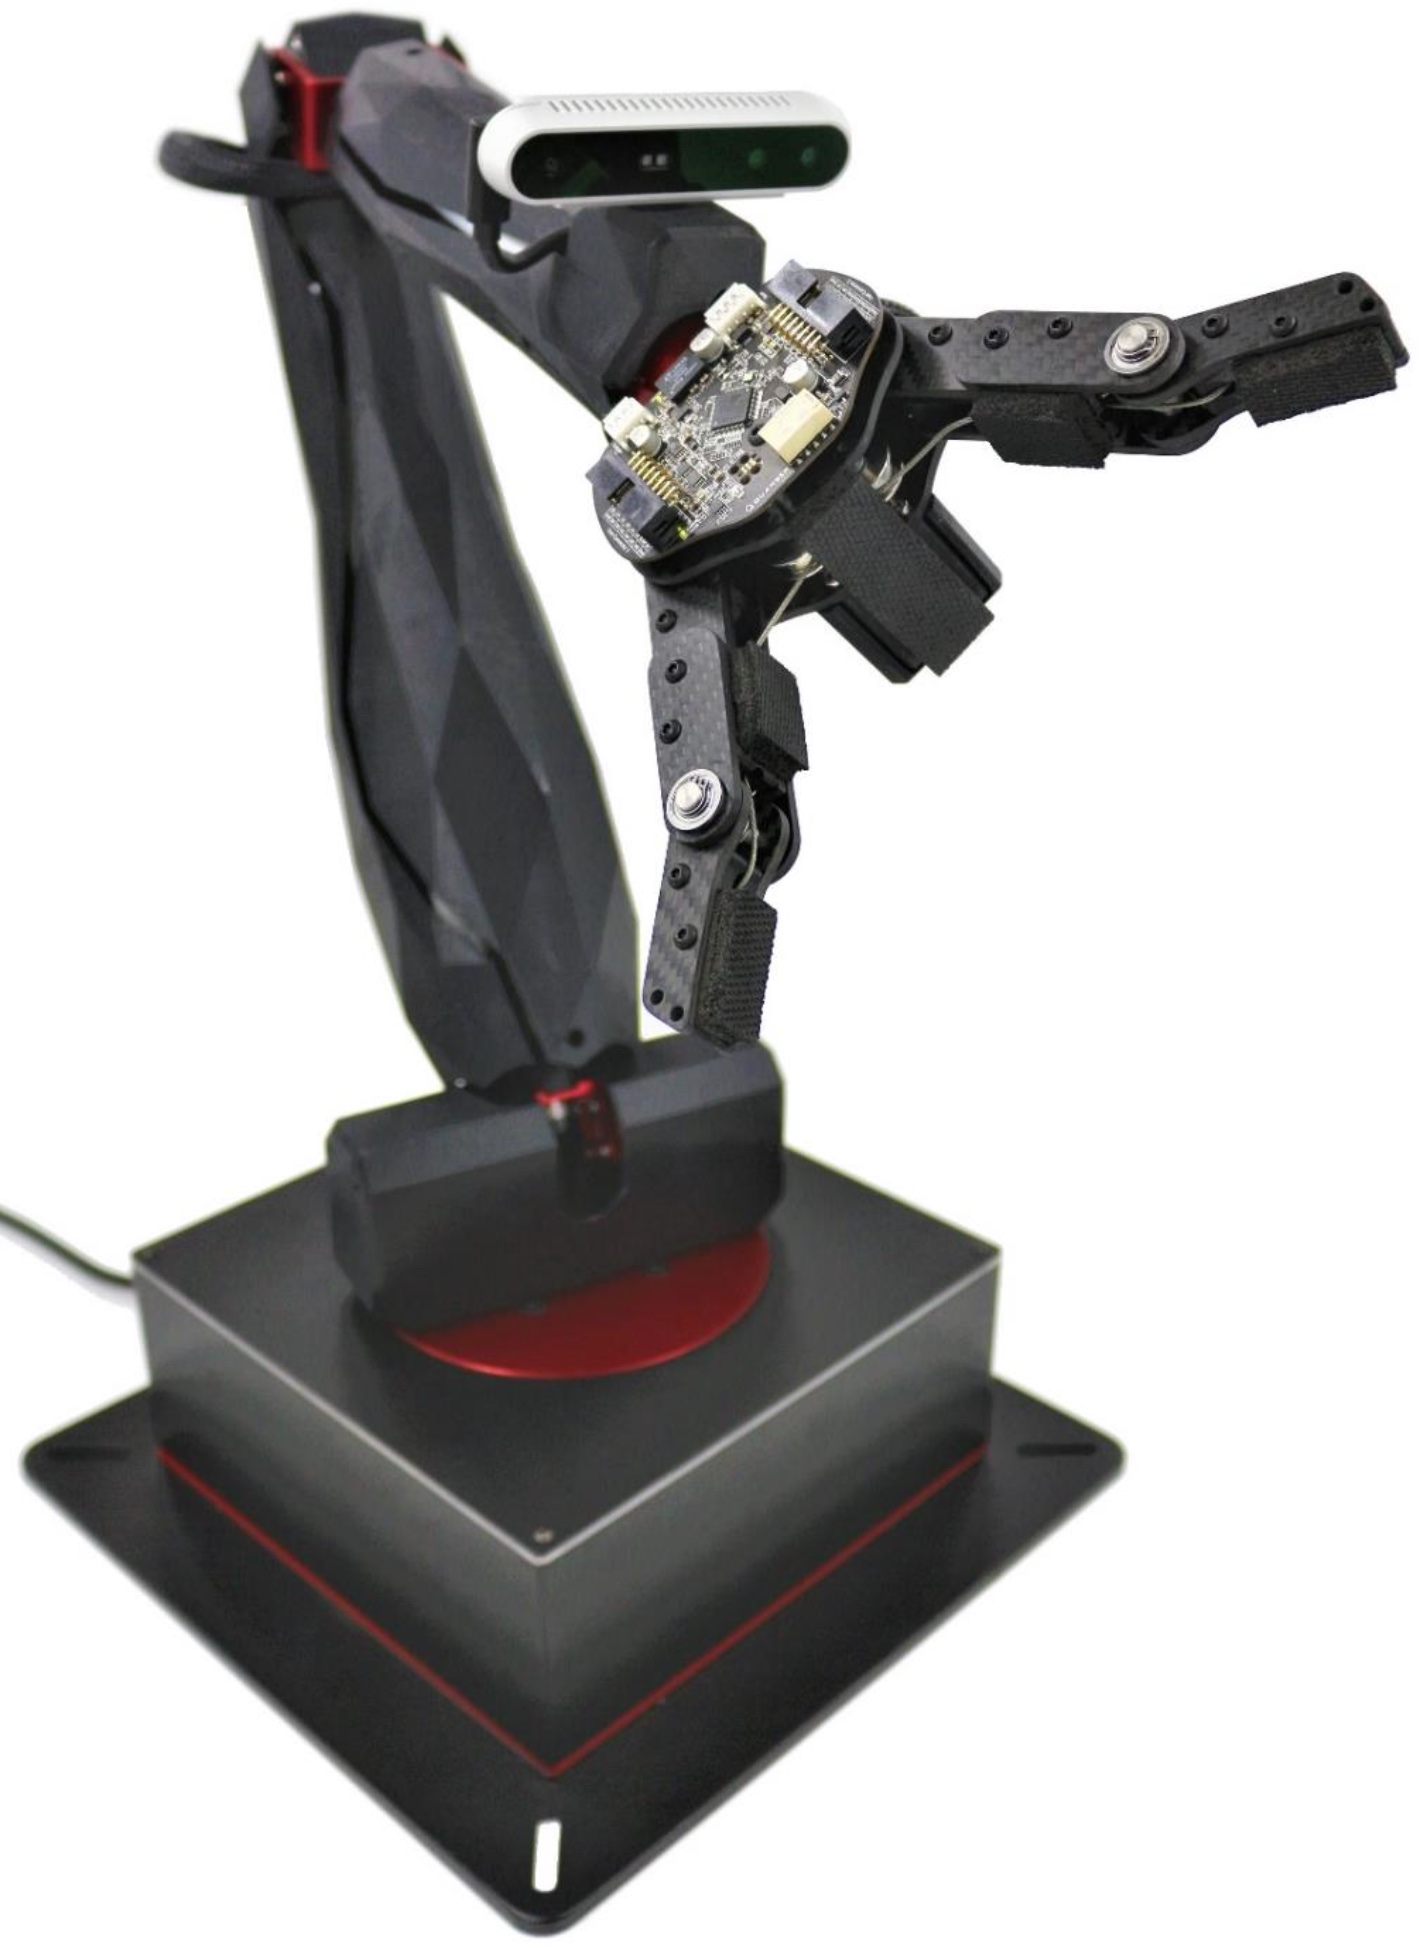
\includegraphics[width=5cm]{Figures/QARM Robot.jpeg}
\caption{Quanser QArm Robot}
\label{fig:QArmPic}
\centering
\end{figure}

